\documentclass[11pt]{article}
\usepackage{fontspec}
\setmainfont{TeX Gyre Pagella}
\usepackage{amsmath,amssymb,amsthm}
\usepackage{geometry}
\geometry{margin=1.1in}
\usepackage{setspace}
\onehalfspacing
\usepackage{enumitem}
\usepackage{longtable}
\usepackage{array}
\usepackage{tikz}
\usetikzlibrary{calc,intersections,arrows.meta,shapes.geometric}
\usepackage[colorlinks=true,linkcolor=black,citecolor=black,urlcolor=black]{hyperref}

\newtheorem{definition}{Definition}
\newtheorem{proposition}{Proposition}
\newtheorem{corollary}{Corollary}
\theoremstyle{remark}
\newtheorem{remark}{Remark}
\newtheorem{example}{Example}

\newcommand{\R}{\mathbb{R}}
\newcommand{\N}{\mathcal{N}}
\newcommand{\id}{\operatorname{id}}
\newcommand{\rank}{\operatorname{rank}}
\newcommand{\E}{\mathbb{E}}
\newcommand{\tv}{\mathrm{TV}}

\title{Holocoordinate Systems:\\ Multidifference Observation, Transition Structure,\\ and Residual Growth in Enriched Atlases}
\author{Flyxion\\ \small Independent Researcher}
\date{September 2026}

\begin{document}
\maketitle

\begin{abstract}
\noindent A coordinate is ordinarily a number, or a vector of numbers, attached to a state. This essay studies a richer object, the \emph{holocoordinate system}: an atlas of perspectives in which each chart carries, besides its local coordinate, a relational signature linking the state to the wider field, translation maps into other perspectives, and a record of the discrepancies the chart fails to explain. Four properties of such a system are formalized and shown to be logically independent: \emph{multidifference completeness}, the requirement that the blind spaces of the charts intersect trivially, characterized through the kernel of the joint differential and quantified by a frame operator; \emph{holography}, the injectivity of a signature on the distinctions to be preserved; \emph{transition consistency}, the cocycle condition on translations; and \emph{holonomy}, the accumulated discrepancy of translation around closed loops of perspectives. Quantitative bounds are given for error amplification under ill-conditioned observation, for cocycle defects and holonomy in terms of pairwise discrepancies, and for the decrease of residuals when a chart is enlarged by a new coordinate, with a martingale limit for the growth rule. An application section treats a tracer-replication instrument as a chart, deriving its blind space, the gauge character of its holonomy under parameter redundancy, and criteria for transporting a fitted coordinate to another perspective. Companion sections state, for each result, what it says and does not say, give worked numerical examples, fix terms and ambiguities, and list common misreadings. A worked example treats a curvilinear quadrilateral construction, in which the relational signature is a pair of ratios along chords, and shows that it determines the point exactly when the frame's coordinates form a chart. The results are conditional on smooth structure that is not assumed to be available for experiential data, and the essay states where that condition bites.
\end{abstract}

\newpage

\section{Introduction}

A coordinate chart on a manifold assigns to each point of an open set a tuple of real numbers, and is the basic device by which a space is made available to calculation. In applied settings the device is often used with less care than in geometry. A chart is taken to have captured a state when its numbers have been recorded, without asking which changes of state leave the numbers unchanged, whether the numbers can be translated into those produced by another chart, or what remains unexplained once the numbers are used. The consequences are familiar from instrument-based measurement: parameters fitted within a model are read as properties of the phenomenon, when they are first of all coordinates of the model.

This essay develops a vocabulary in which those questions have exact answers. The starting point is a state space $X$, assumed to carry the structure of a smooth manifold where derivatives are used, and a family of \emph{perspectives}, each an observation map from a domain in $X$ into a feature space. Three demands are placed on the family.

\begin{enumerate}[label=(\roman*)]
\item \emph{Discrimination.} Every nonzero local difference in $X$ should register in at least one perspective, even if no single perspective registers all of them.
\item \emph{Translation.} The perspectives should retain the means of moving representations between one another, so that agreement, disagreement, and path dependence among them are measurable.
\item \emph{Accountability.} Each perspective should record what it fails to reproduce, so that persistent failure can motivate an enlarged chart rather than being absorbed as noise.
\end{enumerate}

Sections 3 through 6 treat these demands in turn, with a fourth section on signatures that connect a state to the wider field. Section 7 assembles the definitions into an enriched atlas and proves that its component properties are independent, Section 8 applies the vocabulary to a tracer-replication instrument, Section 9 works through a curvilinear quadrilateral construction in which the relational signature can be computed explicitly, and Sections 10 to 13 collect a reading guide, worked numerical examples, a glossary with the ambiguities the essay resolves, and common misreadings. The interest of the construction is partly that independence: a system can discriminate without reconstructing, reconstruct without translating consistently, and translate consistently on every overlap while carrying global holonomy. Keeping the properties separate prevents any one of them from serving as an all-purpose warrant for a coordinate system, in particular the word ``holographic'', which is used here in a reconstructive sense unrelated to the holographic coordinate of high-energy physics (see the remark in Section 4).

The motivating problem, that of coordinates supplied by an instrument whose parameterization may not span the phenomenon, has been discussed in an informal setting elsewhere \cite{flyxion}. What is offered here is the mathematics.

\section*{Plain-language overview}

A coordinate system attaches numbers to states. This essay asks what a system of such numbers can and cannot register, how several systems can be compared, and what a system should do with its own failures. Three questions organize it. Which changes of state does a given measurement fail to register? These are its \emph{blind spaces} (Section 3). How do different measurements of the same states relate, and when do the relations fail to close up? These are \emph{transition maps} and \emph{holonomy} (Section 5). When a measurement mispredicts, what does the failure teach? This is the role of \emph{residuals} (Section 6).

Four properties of a whole system of measurements are separated. \emph{Multidifference completeness} says that no direction of change escapes every measurement at once. \emph{Holography} says that a relational description determines the state it describes. \emph{Transition consistency} says that translations between measurements agree with one another. \emph{Holonomy triviality} says that translating around a closed loop of measurements returns to where it started. The essay shows that none of the four implies another in general, and it gives the sense in which each can be checked separately.

An intuition, with a warning. Take a state that is a position in space and a measurement that reports two of its three coordinates, as an idealized orthographic camera does. Moving toward the camera changes the state and leaves the reading unchanged, so that direction is the blind space. A real perspective camera is not exactly blind to depth, since nearer objects look larger, but it confounds depth with object size, and the same structure reappears in a weaker form. A second camera looking along a different axis removes the blind space. Two cameras looking along almost the same axis remove it only barely, which is the ill-conditioned case of Section 3.

Two cautions apply throughout. First, the results are theorems under stated assumptions and not empirical findings. Several require the state space to be a smooth manifold, which for states of experience or of social systems is a modeling hypothesis, and the illustrations in this essay are illustrations. Second, most results have a narrower reach than a summary suggests. Section~\ref{sec:guide} states, for each result, what it says and what it does not say. Section~\ref{sec:examples} gives worked numerical examples. Section~\ref{sec:terms} fixes terms and lists the ambiguities the essay resolves. Section~\ref{sec:mis} collects common misreadings, several of them arising from the informal summaries above.

\section{Setting}

Let $X$ be a set of states. Where derivatives are used, $X$ is a smooth manifold of dimension $m$; where a probability structure is used, $X$ carries a probability measure $\mu$. A \emph{perspective} is a triple $\alpha=(U_\alpha,V_\alpha,\phi_\alpha)$ consisting of a domain $U_\alpha\subseteq X$, a feature space $V_\alpha$, and an observation map
\[
\phi_\alpha:U_\alpha\longrightarrow V_\alpha .
\]
In Sections 3 and 4, $V_\alpha$ is a finite-dimensional real inner product space, $U_\alpha$ is open, and $\phi_\alpha$ is $C^1$. In Sections 5 and 7, $V_\alpha$ need only be a metric space $(V_\alpha,d_\alpha)$. Different perspectives need not share dimension, variables, or units.

On an overlap $U_{\alpha\beta}=U_\alpha\cap U_\beta$, a \emph{transition map} is a map $T_{\beta\alpha}:V_\alpha\to V_\beta$ intended to satisfy $\phi_\beta=T_{\beta\alpha}\circ\phi_\alpha$ on $U_{\alpha\beta}$. An atlas in the classical sense also requires
\[
T_{\alpha\alpha}=\id,\qquad T_{\alpha\beta}=T_{\beta\alpha}^{-1},\qquad T_{\gamma\beta}\circ T_{\beta\alpha}=T_{\gamma\alpha},
\]
the last being the \emph{cocycle condition}: translating from $\alpha$ to $\gamma$ directly agrees with translating through $\beta$. For observational data the requirements will typically hold only approximately, and the departures are the objects of study.

\section{Blind spaces and multidifference completeness}

Fix $x\in X$ and let $A_x=\{\alpha:x\in U_\alpha\}$, assumed finite.

\begin{definition}[Blind space]
The \emph{blind space} of perspective $\alpha$ at $x$ is
\[
\N_\alpha(x)=\ker D\phi_\alpha(x)\subseteq T_xX .
\]
The \emph{joint blind space} at $x$ is
\[
\N(x)=\bigcap_{\alpha\in A_x}\N_\alpha(x)=\ker D\Phi_x,
\qquad
D\Phi_x(v)=\bigl(D\phi_\alpha(x)v\bigr)_{\alpha\in A_x}.
\]
The family is \emph{multidifference-complete at $x$} when $\N(x)=\{0\}$. In the vocabulary of differential topology this says that the joint observation map $\Phi$ is an immersion at $x$, or is jointly infinitesimally injective.
\end{definition}

A tangent direction $v$ lies in $\N_\alpha(x)$ when motion along $v$ produces no first-order change in perspective $\alpha$. This is the precise sense in which a chart has ``no coordinate'' for a direction: not that no coordinate exists anywhere, but that this observation map is locally insensitive to it. Completeness asks that the insensitivities of different perspectives do not overlap.

\begin{proposition}[Completeness is open and implies local injectivity]\label{prop:open}
The set of points at which the family is multidifference-complete is open. If the family is complete at $x$, there is a neighborhood $W$ of $x$ on which the joint observation map $\Phi=(\phi_\alpha)_{\alpha\in A_x}$ is injective, and $\Phi|_W$ is an embedding into $\bigoplus_{\alpha\in A_x}V_\alpha$.
\end{proposition}

\begin{proof}
Since the $U_\alpha$ are open and $A_x$ is finite, $A_y=A_x$ for $y$ near $x$. Injectivity of the linear map $D\Phi_y$ is equivalent to the nonvanishing of some $m\times m$ minor of its matrix in local coordinates, and this is an open condition because the entries depend continuously on $y$. Completeness at $x$ says that $\Phi$ is an immersion at $x$, and an immersion is locally an embedding by the rank theorem \cite{lee}.
\end{proof}

\begin{remark}
The converse fails. On $X=\R$ the map $\phi(x)=x^3$ is globally injective while $D\phi(0)=0$. First-order blindness at a point indicates degeneracy of the observation at that order, a direction that is ``technically observable but nearly invisible'', not necessarily a failure to distinguish states.
\end{remark}

To quantify how well the perspectives discriminate, equip $T_xX$ with an inner product $g_x$ and each $V_\alpha$ with its inner product $h_\alpha$. Define the \emph{frame operator}
\[
S_x=\sum_{\alpha\in A_x}D\phi_\alpha(x)^{*}D\phi_\alpha(x):T_xX\to T_xX,
\]
where the adjoint is taken with respect to $g_x$ and $h_\alpha$. In the vocabulary of frame theory \cite{christensen}, $S_x$ is the frame operator of the family of linear maps $\{D\phi_\alpha(x)\}$.

\begin{proposition}[Frame characterization]\label{prop:frame}
The operator $S_x$ is self-adjoint and positive semidefinite, with $\langle S_xv,v\rangle=\sum_{\alpha}\|D\phi_\alpha(x)v\|^2$ and $\ker S_x=\N(x)$. Hence the family is complete at $x$ if and only if $S_x$ is positive definite. If $A(x)=\lambda_{\min}(S_x)$ and $B(x)=\lambda_{\max}(S_x)$, then
\[
A(x)\|v\|^2\;\le\;\sum_{\alpha\in A_x}\|D\phi_\alpha(x)v\|^2\;\le\;B(x)\|v\|^2
\qquad(v\in T_xX),
\]
and the stacked Jacobian $J(x)$ has extreme singular values $\sigma_{\min}=\sqrt{A}$, $\sigma_{\max}=\sqrt{B}$. Consequently completeness is equivalent to $\rank J(x)=m$.
\end{proposition}

\begin{proof}
The identity $\langle S_xv,v\rangle=\sum_\alpha\|D\phi_\alpha(x)v\|^2$ follows from the definition of the adjoint. If $S_xv=0$ then this sum vanishes, so $v\in\N(x)$; conversely $v\in\N(x)$ makes each term zero, so $\langle S_xv,v\rangle=0$, and positive semidefiniteness gives $S_xv=0$. The bounds are the Rayleigh bounds for $S_x$. Finally $S_x=J(x)^{*}J(x)$, so the eigenvalues of $S_x$ are the squares of the singular values of $J(x)$.
\end{proof}

Define the \emph{observational condition number}
\[
\kappa_{\mathrm{obs}}(x)=\frac{\sigma_{\max}(J(x))}{\sigma_{\min}(J(x))}=\sqrt{\frac{B(x)}{A(x)}},
\]
with the convention $\kappa_{\mathrm{obs}}=\infty$ when the family is incomplete.

\begin{remark}
The value of $\kappa_{\mathrm{obs}}$ depends on the chosen inner products $g_x$ and $h_\alpha$: rescaling the feature space of one perspective changes the weight with which its differential enters $S_x$. Completeness is invariant under such choices, since it depends only on kernels, but conditioning is not. It should be reported together with the weights, which encode how much each perspective's variables are trusted relative to the others.
\end{remark}

\begin{proposition}[Error amplification]\label{prop:amp}
Suppose the family is complete at $x$ and one observes $y=J(x)v+\eta$ with noise $\eta$, estimating the difference by least squares, $\hat v=J(x)^{+}y$. Then
\[
\|\hat v-v\|\le\frac{\|\eta\|}{\sigma_{\min}(J(x))},
\qquad
\frac{\|\hat v-v\|}{\|v\|}\le\kappa_{\mathrm{obs}}(x)\,\frac{\|\eta\|}{\|J(x)v\|}\quad(v\neq0),
\]
and the first bound is attained for some direction of $\eta$.
\end{proposition}

\begin{proof}
Since $J$ has full column rank, $J^{+}=(J^{*}J)^{-1}J^{*}$ and $J^{+}J=\id$, so $\hat v-v=J^{+}\eta$. The operator norm of $J^{+}$ is $1/\sigma_{\min}(J)$ \cite{golub}, giving the first bound with equality when $\eta$ lies along the left singular vector for $\sigma_{\min}$. For the second, $\|J v\|\le\sigma_{\max}\|v\|$ gives $\|v\|\ge\|Jv\|/\sigma_{\max}$; dividing the first bound by $\|v\|$ yields the claim.
\end{proof}

An ill-conditioned family is therefore one in which some difference is observable in principle and amplified into large uncertainty in practice.

\begin{corollary}[Dimension count]\label{cor:dim}
(i) $\dim\N_\alpha(x)\ge m-\dim V_\alpha$; a perspective with $\dim V_\alpha<m$ therefore has a nonzero blind space. (ii) If the family is complete at $x$, then $\sum_{\alpha\in A_x}\dim V_\alpha\ge m$. (iii) If $\phi_\alpha$ is locally constant near $x$, then $\N_\alpha(x)=T_xX$.
\end{corollary}

\begin{proof}
(i) By rank-nullity, $\dim\ker D\phi_\alpha(x)=m-\rank D\phi_\alpha(x)\ge m-\dim V_\alpha$. (ii) Injectivity of $D\Phi_x:T_xX\to\bigoplus_\alpha V_\alpha$ requires $m\le\sum_\alpha\dim V_\alpha$. (iii) A locally constant map has zero differential.
\end{proof}

Part (iii) applies in particular to perspectives with discrete output, such as a set of category labels, which are locally constant away from category boundaries. First-order completeness cannot be obtained from them.

\section{Relational signatures and reconstruction}

The ``holo'' component of a holocoordinate is a signature that locates a state through its relations to the wider field rather than through independent axes. Let $(X,d)$ be a metric space. A \emph{landmark signature} with landmarks $\ell_1,\dots,\ell_N\in X$ is
\[
\sigma(x)=\bigl(d(x,\ell_1),\dots,d(x,\ell_N)\bigr).
\]
More generally a perspective $\alpha$ may carry a kernel signature $\sigma_\alpha(x)=\int_XK_\alpha(x,y)\Psi(y)\,d\mu(y)$. Such a signature is a compressed description of how the wider field appears from $x$. It is not, without further argument, holographic in any strong sense.

\begin{definition}[Holography]
Let $\sim$ be an equivalence relation on $X$ recording the distinctions one wishes to preserve. A signature $\sigma_\alpha$ is \emph{strongly holographic} (with respect to $\sim$) if
\[
\sigma_\alpha(x)=\sigma_\alpha(y)\ \Longrightarrow\ x\sim y .
\]
A family $\{\sigma_\alpha\}_{\alpha\in A}$ is \emph{jointly holographic} if the joint signature $\Sigma(x)=(\sigma_\alpha(x))_{\alpha\in A}$ has the same property.
\end{definition}

Strong holography is exactly the existence of a reconstruction: a map $G_\alpha$ with $G_\alpha(\sigma_\alpha(x))=[x]$ exists if and only if the implication above holds, and likewise jointly. The following elementary facts separate the two notions.

\begin{proposition}\label{prop:hfacts}
(i) If some $\sigma_\alpha$ is strongly holographic, the family is jointly holographic. (ii) The converse fails: on $X=\R^2$ with $\sigma_1(x)=x_1$ and $\sigma_2(x)=x_2$ and $\sim$ equality, the family is jointly holographic while neither signature is.
\end{proposition}

\begin{proof}
(i) If $\Sigma(x)=\Sigma(y)$ then in particular $\sigma_\alpha(x)=\sigma_\alpha(y)$, so $x\sim y$. (ii) $\Sigma(x)=x$ is injective, while $\sigma_1$ identifies $(x_1,0)$ with $(x_1,1)$.
\end{proof}

In Euclidean space a landmark signature is holographic once enough landmarks are used, and the count is sharp.

\begin{proposition}[Trilateration]\label{prop:tri}
Let $X=\R^m$ with the Euclidean distance and let $\ell_0,\dots,\ell_m$ be affinely independent. Then the landmark signature $\sigma(x)=(\|x-\ell_i\|)_{i=0}^m$ is injective. Fewer than $m+1$ landmarks do not suffice in general.
\end{proposition}

\begin{proof}
Expanding squared distances and subtracting the equation for $i=0$ from that for $i\ge1$ gives the linear system
\[
2(\ell_i-\ell_0)^{\top}x=\|\ell_i\|^2-\|\ell_0\|^2-\sigma_i^2+\sigma_0^2,\qquad i=1,\dots,m.
\]
The rows $(\ell_i-\ell_0)^{\top}$ are linearly independent by affine independence, so the matrix is invertible and $x$ is determined by $\sigma(x)$. With only $m$ landmarks the points $x$ and its reflection across the affine hull of the landmarks have the same signature.
\end{proof}

Injectivity of landmark maps is not automatic in other geometries. On a circle with the arc-length metric, a single landmark cannot separate a point from its reflection through the landmark's axis, while two landmarks that are neither equal nor antipodal do: two distinct reflections composing to a fixed point would force the axes to coincide. Whether a signature is holographic is a property to be verified for the space at hand.

\begin{remark}
If $X$ is compact Hausdorff and $\Sigma$ is continuous and injective, then $\Sigma$ is a homeomorphism onto its image and the reconstruction map is continuous. Without compactness a set-theoretic reconstruction may exist and still be discontinuous.
\end{remark}

\begin{remark}[Terminology]\label{rem:term}
The word ``holographic'' is used here in a purely reconstructive sense: a signature is holographic when it determines the distinctions one wishes to preserve. It is not used in the sense of high-energy physics. In the AdS/CFT correspondence \cite{maldacena} the radial coordinate of anti-de Sitter space, commonly denoted $z$, is called the holographic coordinate. It is a fifth dimension beyond the four of the boundary theory, and its value corresponds to the energy scale at which the boundary theory is probed, with the boundary at small $z$ the ultraviolet regime and large $z$ the infrared \cite{susskind}. Nothing in this essay involves a bulk, a boundary, an additional dimension, or an energy scale, and no coordinate of a holocoordinate system plays the role of $z$. The physics usage refers to a conjectured duality between a gravitational theory and a field theory; nothing analogous is claimed here. A holocoordinate is a chart together with a relational signature, translation maps, and residuals.
\end{remark}

\section{Transition consistency and holonomy}

From here on $V_\alpha$ is a metric space and each $T_{\beta\alpha}:V_\alpha\to V_\beta$ is a globally defined map, assumed Lipschitz with constant $L_{\beta\alpha}$ where a bound is stated. The \emph{transition discrepancy} of a state $x\in U_{\alpha\beta}$ is
\[
\delta_{\alpha\beta}(x)=d_\beta\bigl(\phi_\beta(x),\,T_{\beta\alpha}(\phi_\alpha(x))\bigr).
\]
This is not merely error. Nonzero discrepancy may reflect distortion, information genuinely specific to one perspective, an inadequate transition map, or a missing coordinate; the framework records it without deciding among these. The \emph{cocycle defect} of a triple is
\[
\kappa_{\alpha\beta\gamma}(y)=d_\gamma\bigl(T_{\gamma\beta}T_{\beta\alpha}y,\;T_{\gamma\alpha}y\bigr),\qquad y\in V_\alpha .
\]

\begin{proposition}[Cocycle defect from discrepancies]\label{prop:cocycle}
For $x\in U_\alpha\cap U_\beta\cap U_\gamma$ and $y=\phi_\alpha(x)$,
\[
\kappa_{\alpha\beta\gamma}(y)\;\le\;L_{\gamma\beta}\,\delta_{\alpha\beta}(x)+\delta_{\beta\gamma}(x)+\delta_{\alpha\gamma}(x).
\]
In particular, if all discrepancies vanish, the cocycle condition holds at $\phi_\alpha(x)$.
\end{proposition}

\begin{proof}
By the triangle inequality in $V_\gamma$,
\begin{align*}
\kappa_{\alpha\beta\gamma}(y)
&\le d_\gamma\bigl(T_{\gamma\beta}T_{\beta\alpha}y,\,T_{\gamma\beta}\phi_\beta(x)\bigr)
+d_\gamma\bigl(T_{\gamma\beta}\phi_\beta(x),\,\phi_\gamma(x)\bigr)
+d_\gamma\bigl(\phi_\gamma(x),\,T_{\gamma\alpha}y\bigr).
\end{align*}
The first term is at most $L_{\gamma\beta}\,d_\beta(T_{\beta\alpha}y,\phi_\beta(x))=L_{\gamma\beta}\delta_{\alpha\beta}(x)$, the second is $\delta_{\beta\gamma}(x)$, and the third is $\delta_{\alpha\gamma}(x)$.
\end{proof}

Now consider a loop of perspectives $\alpha_0\to\alpha_1\to\cdots\to\alpha_k=\alpha_0$ and write $T_i=T_{\alpha_{i+1}\alpha_i}$ with Lipschitz constants $L_i$. The \emph{holonomy map} of the loop is
\[
\mathcal H_\gamma=T_{k-1}\circ\cdots\circ T_1\circ T_0:V_{\alpha_0}\to V_{\alpha_0}.
\]
For a state $x$ lying in every $U_{\alpha_i}$, the \emph{holonomy discrepancy} is
\[
\Omega_\gamma(x)=d_{\alpha_0}\bigl(\phi_{\alpha_0}(x),\,\mathcal H_\gamma(\phi_{\alpha_0}(x))\bigr).
\]

\begin{proposition}[Holonomy bound]\label{prop:holbound}
For $x\in\bigcap_{i}U_{\alpha_i}$, writing $\delta_j=\delta_{\alpha_j\alpha_{j+1}}(x)$,
\[
\Omega_\gamma(x)\;\le\;\sum_{j=0}^{k-1}\Bigl(\prod_{l=j+1}^{k-1}L_l\Bigr)\delta_j .
\]
In particular $\Omega_\gamma(x)>0$ implies $\delta_j(x)>0$ for some $j$, and a loop over a common state has trivial holonomy discrepancy whenever the discrepancies vanish.
\end{proposition}

\begin{proof}
Let $z_i=\phi_{\alpha_i}(x)$ and define $y_0=z_0$, $y_{i+1}=T_i(y_i)$, so that $y_k=\mathcal H_\gamma(z_0)$ and $z_k=z_0$. We show by induction that
\[
d_{\alpha_i}(y_i,z_i)\le\sum_{j<i}\Bigl(\prod_{l=j+1}^{i-1}L_l\Bigr)\delta_j .
\]
For $i=0$ both sides are zero. Given the bound at $i$,
\[
d(y_{i+1},z_{i+1})\le d(T_iy_i,T_iz_i)+d(T_iz_i,z_{i+1})\le L_i\,d(y_i,z_i)+\delta_i,
\]
and substituting the inductive bound gives the bound at $i+1$. Taking $i=k$ and using $\Omega_\gamma(x)=d_{\alpha_0}(z_k,y_k)$ completes the proof.
\end{proof}

The bound runs one way. Discrepancies may cancel around a loop, so vanishing holonomy does not imply vanishing discrepancy: holonomy detects the part of the discrepancy that survives transport, and is a coarser instrument than the pairwise discrepancies themselves. Around a triangle the relation to the cocycle condition is exact.

\begin{proposition}[Triangle holonomy]\label{prop:trihol}
Suppose $T_{\alpha\gamma}=T_{\gamma\alpha}^{-1}$ with $T_{\gamma\alpha}$ bijective, and let
\[
H=T_{\alpha\gamma}T_{\gamma\beta}T_{\beta\alpha}.
\]
Then for $y\in V_\alpha$, $H(y)=y$ if and only if $\kappa_{\alpha\beta\gamma}(y)=0$.
\end{proposition}

\begin{proof}
$H(y)=y$ holds if and only if $T_{\gamma\alpha}^{-1}(T_{\gamma\beta}T_{\beta\alpha}y)=y$, that is, if and only if $T_{\gamma\beta}T_{\beta\alpha}y=T_{\gamma\alpha}y$.
\end{proof}

Loops that are not products of triangles are not controlled by the cocycle conditions. The following example shows that exact charts can carry nontrivial holonomy even though every cocycle condition holds.

\begin{example}[Winding on the circle]\label{ex:winding}
Let $X=\R/2\pi\mathbb Z$ and choose $0<\varepsilon<\pi/3$. Cover $X$ by three arcs $U_1=(-\varepsilon,\tfrac{2\pi}{3}+\varepsilon)$, $U_2=(\tfrac{2\pi}{3}-\varepsilon,\tfrac{4\pi}{3}+\varepsilon)$, $U_3=(\tfrac{4\pi}{3}-\varepsilon,2\pi+\varepsilon)$, with $\phi_\alpha:U_\alpha\to\R$ the angle read in the stated interval. The overlaps $U_{12}$, $U_{23}$, $U_{13}$ are nonempty and there are no triple overlaps. Take $T_{21}=T_{32}=\id_\R$ and $T_{31}(y)=y+2\pi$, which agree with $\phi_\beta\circ\phi_\alpha^{-1}$ on the overlaps, the last because a point near $0$ has angle in $(-\varepsilon,\varepsilon)$ in chart 1 and in $(2\pi-\varepsilon,2\pi+\varepsilon)$ in chart 3. Every chart is an exact coordinate and every cocycle condition is vacuous, yet for the loop $1\to2\to3\to1$,
\[
\mathcal H=T_{13}\circ T_{32}\circ T_{21}=T_{31}^{-1},\qquad \mathcal H(y)=y-2\pi\neq y .
\]
The holonomy is the winding number of the circle, invisible to every chart and to every triple of charts.
\end{example}

\begin{remark}[Cohomological classification]\label{rem:coh}
Suppose the transition maps are invertible, take values in a group $G$ acting on a common feature space (for instance translations or affine maps), and satisfy the cocycle condition on every nonempty triple overlap. Then $\{T_{\beta\alpha}\}$ is a \v{C}ech $1$-cocycle on the nerve $\mathcal{K}$ of the cover with values in $G$. Its class in $\check H^1(\mathcal K;G)$ vanishes if and only if there are $g_\alpha\in G$ with $T_{\beta\alpha}=g_\beta g_\alpha^{-1}$, that is, if and only if the charts can be renormalized by $\phi_\alpha\mapsto g_\alpha^{-1}\phi_\alpha$ so that every transition map becomes the identity. For connected $\mathcal K$ the classes correspond to $\mathrm{Hom}(\pi_1(\mathcal K),G)/G$, the class being the holonomy representation, so holonomy around every loop is trivial exactly when the class is trivial. When $\mathcal K$ is simply connected the class vanishes for every $G$, which is why the triangle conditions then control everything. In Example~\ref{ex:winding} the nerve is the boundary of a triangle with $\pi_1=\mathbb Z$, $G=(\R,+)$, and the class is $2\pi\in\check H^1(\mathcal K;\R)=\R$. For nonabelian $G$ the set $\check H^1$ is a pointed set rather than a group \cite{bott}. Transition maps that are merely Lipschitz, without a group structure, are not covered by this classification.
\end{remark}

\section{Residuals and the growth rule}

A perspective can also be held to account for what it fails to reproduce. Let $P_q:X\to\R$ be a family of square-integrable \emph{probes} $q\in Q$ extracting properties from a state, and let $\phi_\alpha$ be a chart whose output is used to predict them. With squared error, the best decoder of probe $q$ from the chart is the conditional expectation, and the \emph{residual} is
\[
\varepsilon_{\alpha,q}(x)=P_q(x)-\E\bigl[P_q\mid\phi_\alpha\bigr](x),
\qquad
\varepsilon_\alpha=(\varepsilon_{\alpha,q})_{q\in Q}.
\]
Enlarging the chart by a measurable function $z$ of the state gives $\tilde\phi_\alpha=(\phi_\alpha,z)$ and the enlarged residual $\tilde\varepsilon_{\alpha,q}=P_q-\E[P_q\mid\phi_\alpha,z]$.

\begin{proposition}[Residual reduction]\label{prop:resid}
For each probe,
\[
\E\bigl[\tilde\varepsilon_{\alpha,q}^{\,2}\bigr]
=\E\bigl[\varepsilon_{\alpha,q}^{\,2}\bigr]
-\E\Bigl[\bigl(\E[P_q\mid\phi_\alpha,z]-\E[P_q\mid\phi_\alpha]\bigr)^2\Bigr].
\]
Hence enlargement never increases the mean squared residual, and decreases it strictly if and only if $\E[P_q\mid\phi_\alpha,z]\neq\E[P_q\mid\phi_\alpha]$ on a set of positive measure, that is, if and only if the residual is \emph{structured} with respect to $z$.
\end{proposition}

\begin{proof}
Write $P=P_q$, $F=\sigma(\phi_\alpha)$, $\tilde F=\sigma(\phi_\alpha,z)\supseteq F$. Then
\[
P-\E[P\mid F]=\bigl(P-\E[P\mid\tilde F]\bigr)+\bigl(\E[P\mid\tilde F]-\E[P\mid F]\bigr).
\]
The two summands are orthogonal in $L^2$: the first is orthogonal to every $\tilde F$-measurable square-integrable function, and the second is $\tilde F$-measurable. Taking second moments gives the identity.
\end{proof}

This yields the growth rule
\[
\begin{aligned}
&\text{observe}\to\text{translate}\to\text{detect residual}\\
&\qquad\to\text{differentiate residual}\to\text{add coordinate}
\end{aligned}
\]
a quantitative form. A residual that is unstructured, in the sense that $\E[\varepsilon_{\alpha,q}\mid\phi_\alpha,z]=0$ for every candidate $z$, cannot be reduced by any enlargement.

\begin{corollary}[Limit of the growth rule]\label{cor:growth}
Let $z_1,z_2,\dots$ be successively added coordinates and $\mathcal F_n=\sigma(\phi_\alpha,z_1,\dots,z_n)$, $\mathcal F_\infty=\sigma(\bigcup_n\mathcal F_n)$. Then the mean squared residual is nonincreasing in $n$ and converges to $\E[(P_q-\E[P_q\mid\mathcal F_\infty])^2]$. The limit is zero if and only if $P_q$ is $\mathcal F_\infty$-measurable almost surely.
\end{corollary}

\begin{proof}
Monotonicity is the previous proposition. Convergence of $\E[P_q\mid\mathcal F_n]$ to $\E[P_q\mid\mathcal F_\infty]$ in $L^2$ is L\'evy's upward theorem \cite{williams}, and the last statement follows because a function equals its conditional expectation on $\mathcal F_\infty$ exactly when it is $\mathcal F_\infty$-measurable.
\end{proof}

\begin{remark}
The statement is population-level. With finite data, enlargement can fit noise, and detecting a structured residual requires held-out probes; no claim is made here about estimation.
\end{remark}

\section{Enriched atlases and the independence of their properties}

\begin{definition}[Holocoordinate system]\label{def:holo}
A \emph{holocoordinate system} on $X$ is an enriched atlas
\[
\mathfrak H=\bigl\{(U_\alpha,\phi_\alpha,\sigma_\alpha,T_{\beta\alpha},\varepsilon_\alpha)\bigr\}_{\alpha\in A},
\]
in which $\phi_\alpha$ is a local coordinate, $\sigma_\alpha$ is a relational signature, $T_{\beta\alpha}$ transports representations between perspectives, and $\varepsilon_\alpha$ records the residuals of the chart. For a designated set $A_0\subseteq A$ of perspectives, $\mathfrak H$ is
\begin{itemize}[nosep]
\item[\textbf{(M)}] \emph{multidifference-complete at $x$} if $\N(x)=\{0\}$;
\item[\textbf{(H)}] \emph{strongly holographic} if $\sigma_\alpha$ is strongly holographic for every $\alpha\in A_0$;
\item[\textbf{(C)}] \emph{transition-consistent} if $\delta_{\alpha\beta}\equiv0$ on every overlap and all cocycle conditions hold;
\item[\textbf{(V)}] \emph{holonomy-trivial} if every holonomy map is the identity on its domain.
\end{itemize}
\end{definition}

\begin{proposition}[Independence]\label{prop:indep}
None of the following implications holds in general.
\begin{enumerate}[label=(\alph*),nosep]
\item \textbf{(M)} does not imply \textbf{(H)}.
\item \textbf{(H)} does not imply \textbf{(C)}.
\item \textbf{(C)} does not imply \textbf{(V)}.
\item \textbf{(V)} does not imply \textbf{(C)}.
\item \textbf{(C)} does not imply \textbf{(M)}, and \textbf{(H)} does not imply \textbf{(M)}.
\end{enumerate}
\end{proposition}

\begin{proof}
(a) The family $\phi_1=x_1$, $\phi_2=x_2$ on $\R^2$ with $\sigma_\alpha=\phi_\alpha$ is complete, since $D\Phi=\id$, while neither signature is strongly holographic. (b) On $X=\R$ take three charts with $\phi_\alpha=\id$, $\sigma_\alpha=\id$ (injective), $T_{21}=T_{32}=\id$ and $T_{31}(y)=y+1$. Then $\kappa_{123}\equiv1$ and $\delta_{13}\equiv1$. (c) Example~\ref{ex:winding}: every chart is exact and all cocycle conditions hold vacuously, but the holonomy is a nonzero translation. (d) Take two charts $\phi_1=\phi_2=\id$ on $\R$ with $T_{21}(y)=y+1$ and $T_{12}=T_{21}^{-1}$. The loop $1\to2\to1$ is the identity, yet $\delta_{12}\equiv1$. (e) A single chart $\phi(x)=x_1$ on $\R^2$ satisfies \textbf{(C)} and \textbf{(V)} vacuously and fails \textbf{(M)}; a constant chart $\phi\equiv0$ with $\sigma=\id$ satisfies \textbf{(H)} and fails \textbf{(M)}.
\end{proof}

The independence is the point of the construction. A system can observe every difference without reconstructing the state (a), reconstruct without translating consistently (b), be exact on every overlap while carrying global holonomy (c), close every loop without being consistent (d), and be consistent or reconstructive while blind to some directions (e). Each property is separately testable, and a claim that a system is ``holographic'' is accordingly a claim about signature injectivity and nothing else.

\section{Application: the tracer replication chart}

The preceding vocabulary applies to any instrument that converts a compressed parameter vector into an exposed rendering which a participant compares with an experience. The Tracer Replication Tool discussed in \cite{flyxion} and \cite{qri_note} is such an instrument. This section uses it as an illustration and makes no claim about any data collected with it.

\paragraph{Modeling assumptions.} (A1) The experiences of interest form a smooth $m$-manifold $X$. (A2) Comparison is mediated by a finite-dimensional Euclidean feature space $W$, with a smooth map $\iota:X\to W$ giving the features of an experience and a smooth renderer $R:\Theta\to W$, $\Theta\subseteq\R^p$ open, giving the features of the pattern produced by a parameter vector (persistence, intensity, decay, strobe frequency, replay frequency, pulse, envelope parameters, color inversion). (A3) The comparison functional is squared distance, $D_e(w)=\|\iota(e)-w\|^2$. These are strong simplifications. The subjective comparison of the participant need not be a metric, and (A1) is the smoothness hypothesis flagged in Section~\ref{sec:scope}.

Suppose first that $R$ is an embedding of $\Theta$ onto a submanifold $M=R(\Theta)\subseteq W$ of dimension $p$, and that $\mathcal T$ is a tubular neighborhood of $M$ with smooth nearest-point retraction $\pi:\mathcal T\to M$. For $\iota(e)\in\mathcal T$ the fitted parameter is unique, and the \emph{tool chart} is
\[
\phi_\tau(e)=R^{-1}\bigl(\pi(\iota(e))\bigr)\in\Theta .
\]

\begin{proposition}[Blind space of the tool chart]\label{prop:toolblind}
If $\iota$ is an immersion at $e$, then
\[
\N_\tau(e)=\bigl\{v\in T_eX:\ D\iota(e)v\in N_{\pi(\iota(e))}M\bigr\},
\]
where $N_qM$ is the normal space of $M$ at $q$. Consequently $\dim\N_\tau(e)\ge m-p$.
\end{proposition}

\begin{proof}
By the tubular neighborhood theorem $\pi$ is a submersion whose fibers are the normal disks, so $\ker D\pi_w=N_{\pi(w)}M$. Since $R^{-1}:M\to\Theta$ is a diffeomorphism, $D\phi_\tau(e)=D(R^{-1})\circ D\pi\circ D\iota(e)$ has the kernel stated. Because $D\iota(e)$ is injective, $\dim\N_\tau(e)=\dim\bigl(D\iota(e)(T_eX)\cap N_qM\bigr)$, and two subspaces of $W$ of dimensions $m$ and $\dim W-p$ meet in dimension at least $m+(\dim W-p)-\dim W=m-p$.
\end{proof}

The blind space of the tool chart is thus the set of changes in experience whose perceptual image is normal to the model manifold: exactly the variation for which the parameterization has no coordinate. If $m>p$ the tool chart cannot be complete on its own (Corollary~\ref{cor:dim}), and completeness must come from other perspectives whose blind spaces meet the tool's only at zero.

\paragraph{From embedding to degeneracy.} Proposition 11 assumes that $R$ is an embedding. The behavior of the tool chart depends on how far $R$ departs from that, and three regimes should be distinguished.
\begin{enumerate}[label=(\arabic*),nosep]
\item \emph{Embedding.} The fit is unique near $\iota(e)$ and the blind space is given by Proposition 11.
\item \emph{Immersion that is not injective.} Locally $R$ is still an embedding, so on each small sheet Proposition 11 applies, but the sheets can overlap or wrap, and the fitted parameter is multivalued. The chart exists only on branches, and the blind space is a property of the branch.
\item \emph{Rank drop.} $DR(\theta)$ has a kernel, the fibers of $R$ have positive dimension, and the chart takes values in a quotient, as discussed below.
\end{enumerate}

\begin{proposition}[Branch dependence of the blind space]\label{prop:branch}
Let $R$ be an immersion, let $\theta_0\neq\theta_1$ satisfy $R(\theta_0)=R(\theta_1)=\iota(e)=q$, and choose neighborhoods $\Theta_j\ni\theta_j$ on which $R$ is an embedding, with images $M_j$ admitting tubular retractions $\pi_j$ near $q$. Let $\phi^{(j)}(e')=(R|_{\Theta_j})^{-1}(\pi_j(\iota(e')))$ be the corresponding branch charts. If $\iota$ is an immersion at $e$, then
\[
\N^{(j)}(e)=D\iota(e)^{-1}\bigl(N_qM_j\bigr),\qquad j=0,1.
\]
In particular, if $T_qM_0=T_qM_1$ the two blind spaces coincide. In general they need not.
\end{proposition}

\begin{proof}
Apply Proposition 11 to each sheet. Equal tangent spaces have equal orthogonal complements in $W$, so the preimages coincide. For a failure of coincidence, take $X=W=\R^2$, $\iota=\id$, and two sheets crossing transversally at $q$: the blind spaces are the two distinct normal lines.
\end{proof}

\begin{example}[Monodromy in the tool setting]\label{ex:mono}
Let $\Theta=\R$, $W=\R^2$, $R(\theta)=(\cos\theta,\sin\theta)$, $X=W\setminus\{0\}$ and $\iota$ the inclusion, so $m=2$, $p=1$. Then $R$ is an immersion but not injective, $M$ is the unit circle, and the fitted parameter of an experience $e$ is its argument, determined only modulo $2\pi$. On each branch the blind space is the radial line, by Proposition 11. Continuing a branch chart along the loop $e(t)=(\cos t,\sin t)$, $t\in[0,2\pi]$, returns the parameter $\theta+2\pi$, so the holonomy is translation by $2\pi$, which is Example~\ref{ex:winding} realized inside the instrument. No continuous single-valued choice of parameter exists over the loop, since one would be a continuous lift of the argument map on the circle to the covering $\R\to S^1$. The obstruction disappears only if the chart is allowed to take values in the quotient $\Theta/{\sim_R}\cong S^1$, that is, only if the linear coordinate is given up.
\end{example}

\paragraph{Parameter redundancy.} Suppose instead that $R$ is not an immersion, so that distinct parameter vectors can produce indistinguishable outputs. Write $\theta\sim_R\theta'$ when $R(\theta)=R(\theta')$. The fitted parameter is then determined only up to $\sim_R$, and the tool chart takes values in the quotient $\Theta/{\sim_R}$. A function $f:\Theta\to\R$ is a well-defined function of the chart only if it respects the quotient.

\begin{proposition}[Well-defined coordinate functions]\label{prop:wellfn}
A function $f:\Theta\to\R$, such as a fitted replay frequency, descends to a function on the chart values $\Theta/{\sim_R}$ if and only if $f$ is constant on the fibers of $R$. In particular, exhibiting $\theta,\theta'$ with $R(\theta)=R(\theta')$ and $f(\theta)\ne f(\theta')$ shows that $f(\theta^\ast)$ is not determined by what the tool distinguishes.
\end{proposition}

\begin{proof}
A function on a quotient is precisely a function constant on equivalence classes, and the classes of $\sim_R$ are the fibers of $R$.
\end{proof}

\begin{example}[Holonomy as gauge]
Let $s:R(\Theta)\to\Theta$ be a selection of one representative from each fiber, and consider the loop that renders a parameter vector, refits, and reads the parameters again: $\theta\mapsto R(\theta)\mapsto s(R(\theta))$. The holonomy discrepancy is $\Omega(\theta)=d(\theta,s(R(\theta)))$, which is positive exactly when $\theta$ is not the selected representative. It vanishes identically for the quotient chart. This holonomy is a coordinate artifact: it depends on the choice of $s$ and disappears in $\Theta/{\sim_R}$. It differs in kind from the winding of Example~\ref{ex:winding} and the monodromy of Example~\ref{ex:mono}, which cannot be removed by recoordinatizing the charts.
\end{example}

\paragraph{Categorical and graded reports.} Verbal categories such as \emph{trail}, \emph{strobe}, and \emph{replay} form a perspective with discrete output. By Corollary~\ref{cor:dim}(iii) such a perspective has full blind space wherever it is differentiable, and registers change only when a state crosses a category boundary. It can be handled by the metric machinery of Section~5 but contributes nothing to first-order completeness. Graded ratings on continuous scales do contribute, and a complete family in practice requires perspectives of that kind.

\paragraph{Transporting a fitted coordinate to a process.} A value of $\phi_\tau$ is a coordinate of the tool chart. To assert that it corresponds to a process in another substrate, say a feature vector $\phi_\nu$ of recorded neural activity, requires a transition map $T_{\nu\tau}$ and evidence about it. In the vocabulary of Sections 5 and 7 the assertion is supported to the extent that:
\begin{enumerate}[label=(\roman*),nosep]
\item the discrepancy $\delta_{\tau\nu}(e)$ is small on held-out states, that is, the map predicts the second perspective rather than being fitted to it;
\item cocycle defects $\kappa_{\tau\nu\gamma}$ are small with respect to further perspectives $\gamma$, such as psychophysical or behavioral charts, so that the correspondence is not particular to one pair;
\item the joint family is complete at the states in question, so that the agreement is not carried entirely by directions in which some chart is blind; and
\item the transported quantity is a well-defined function of the chart in the sense of the last proposition.
\end{enumerate}
A fitted replay frequency that satisfies none of these establishes that a replay at that frequency in the renderer resembles a remembered experience, and nothing further.

\paragraph{Contaminated growth.} Proposition~\ref{prop:resid} compares residuals under a fixed joint law of probes and chart outputs. If exposure to the tool changes how experiences are recalled and reported, the law after $k$ exposures, $\mu_k$, differs from $\mu_{k-1}$, and mean squared residuals computed under different laws are not comparable: a decrease may reflect changed reports rather than an added coordinate. The identity of Proposition~\ref{prop:resid} remains valid at each fixed $k$, and the growth rule remains meaningful if the probes are elicited, or the residuals evaluated, under a fixed reference law, for instance from reports collected before exposure. A candidate new coordinate $z$, such as a graded rating of spatial coherence of the trails that the tool does not parameterize, is supported when $\E[P_q\mid\phi_\tau,z]\ne\E[P_q\mid\phi_\tau]$ under that reference law, and not merely when participants report wanting a further control.

\section{A curvilinear worked example: the quadrilateral construction}\label{sec:quad}

The vocabulary of the preceding sections can be exercised on a construction simple enough to compute by hand: a curvilinear quadrilateral whose four sides carry extreme coordinate values, with a point located by ratios along two chords. It is a form of linear interpolation along chords between boundary curves, in the spirit of transfinite interpolation of Coons type \cite{coons}, and it is stated here on its own terms (Figure~\ref{fig:quad}).

\paragraph{Setting.} Let $\Omega\subset\R^2$ be a compact region bounded by four curves: a bottom side $\Gamma_-$ on which $\varphi=\varphi_-$, a top side $\Gamma_+$ on which $\varphi=\varphi_+$, a left side $\Gamma_{\mathrm l}$ on which $\lambda=\lambda_-$, and a right side $\Gamma_{\mathrm r}$ on which $\lambda=\lambda_+$, with $\varphi_-<\varphi_+$ and $\lambda_-<\lambda_+$. Let $(\lambda,\varphi):\Omega\to R=[\lambda_-,\lambda_+]\times[\varphi_-,\varphi_+]$ be continuous. A \emph{chord rule} assigns to each $P\in\Omega$ a vertical chord $[A,B]\ni P$ with $A\in\Gamma_-$ and $B\in\Gamma_+$, and a horizontal chord $[C,D]\ni P$ with $C\in\Gamma_{\mathrm l}$ and $D\in\Gamma_{\mathrm r}$, where chords are straight segments contained in $\Omega$. The \emph{relational signature} of $P$ is
\[
h(P)=(u,v)=\Bigl(\frac{AP}{AB},\ \frac{DP}{CD}\Bigr)\in[0,1]^2,
\]
with Euclidean lengths, the first ratio measured from the bottom end and the second from the right end. The \emph{interpolated coordinates} are
\[
\tilde\varphi(P)=\varphi_-+u\,(\varphi_+-\varphi_-),\qquad
\tilde\lambda(P)=\lambda_+-v\,(\lambda_+-\lambda_-).
\]
Equivalently, $\Delta\varphi=(\varphi_+-\varphi_-)\,AP/AB$ and $\Delta\lambda=(\lambda_+-\lambda_-)\,DP/CD$ are the offsets $\tilde\varphi-\varphi_-$ and $\lambda_+-\tilde\lambda$. The sign convention matters: $v$ is measured from the right side, so the interpolated $\lambda$ is $\lambda_+-\Delta\lambda$ and not $\lambda_-+\Delta\lambda$.

The interpolated coordinates are the frame-relative perspective translated into the coordinate perspective, and their departure from the true coordinates is a transition discrepancy in the sense of Section 5. Figure~\ref{fig:quad} shows the construction.

\begin{figure}[!htbp]
\centering
\newcommand{\bezpt}[6]{\coordinate (#1) at ($ {(1-#6)^3}*(#2)+{3*(1-#6)^2*#6}*(#3)+{3*(1-#6)*#6^2}*(#4)+{#6^3}*(#5) $);}
\begin{tikzpicture}[scale=0.85,>=Stealth,
  bnd/.style={thick},
  fam/.style={gray!55,thin},
  chord/.style={dashed,thick},
  pt/.style={circle,fill,inner sep=1.3pt}]
  % boundary data
  \coordinate (G) at (0,0);   \coordinate (E) at (9,0.6);
  \coordinate (H) at (0.5,6); \coordinate (F) at (8.6,6.6);
  \coordinate (bc1) at (3,-0.6);   \coordinate (bc2) at (6,1.3);
  \coordinate (tc1) at (3.2,5.5);  \coordinate (tc2) at (6,7.2);
  \coordinate (lc1) at (-0.6,2);   \coordinate (lc2) at (1.2,4);
  \coordinate (rc1) at (9.6,2.5);  \coordinate (rc2) at (8,4.5);
  % schematic coordinate families
  \foreach \s [count=\i] in {0.2,0.4,0.6,0.8}{
    \bezpt{L\i}{G}{lc1}{lc2}{H}{\s}
    \bezpt{R\i}{E}{rc1}{rc2}{F}{\s}
    \coordinate (fa\i) at ($ {1-\s}*(bc1)+{\s}*(tc1) $);
    \coordinate (fb\i) at ($ {1-\s}*(bc2)+{\s}*(tc2) $);
    \draw[fam] (L\i) .. controls (fa\i) and (fb\i) .. (R\i);
    \bezpt{Bt\i}{G}{bc1}{bc2}{E}{\s}
    \bezpt{Tt\i}{H}{tc1}{tc2}{F}{\s}
    \coordinate (ga\i) at ($ {1-\s}*(lc1)+{\s}*(rc1) $);
    \coordinate (gb\i) at ($ {1-\s}*(lc2)+{\s}*(rc2) $);
    \draw[fam] (Bt\i) .. controls (ga\i) and (gb\i) .. (Tt\i);
  }
  % boundary
  \draw[bnd] (G) .. controls (bc1) and (bc2) .. (E)
             .. controls (rc1) and (rc2) .. (F)
             .. controls (tc2) and (tc1) .. (H)
             .. controls (lc2) and (lc1) .. (G);
  % chord endpoints and intersection
  \bezpt{A}{G}{bc1}{bc2}{E}{0.55}
  \bezpt{B}{H}{tc1}{tc2}{F}{0.62}
  \bezpt{C}{G}{lc1}{lc2}{H}{0.42}
  \bezpt{D}{E}{rc1}{rc2}{F}{0.5}
  \path[name path=chAB] (A)--(B);
  \path[name path=chCD] (C)--(D);
  \path[name intersections={of=chAB and chCD,by=P}];
  \draw[chord] (A)--(B);
  \draw[chord] (C)--(D);
  \foreach \q in {A,B,C,D,P}{\node[pt] at (\q) {};}
  % labels
  \node[below left] at (G) {$G$};  \node[below right] at (E) {$E$};
  \node[above left] at (H) {$H$};  \node[above right] at (F) {$F$};
  \node[below] at (A) {$A$};       \node[above] at (B) {$B$};
  \node[left] at (C) {$C$};        \node[right] at (D) {$D$};
  \node[above right,inner sep=2pt] at (P) {$P$};
  \path (G) .. controls (bc1) and (bc2) .. (E) node[pos=0.17,below=3pt] {$\varphi=\varphi_-$};
  \path (H) .. controls (tc1) and (tc2) .. (F) node[pos=0.2,above=3pt] {$\varphi=\varphi_+$};
  \path (G) .. controls (lc1) and (lc2) .. (H) node[pos=0.75,left=3pt] {$\lambda=\lambda_-$};
  \path (E) .. controls (rc1) and (rc2) .. (F) node[pos=0.8,right=3pt] {$\lambda=\lambda_+$};
  \node[font=\small,right=2pt] at ($(A)!0.5!(P)$) {$AP$};
  \node[font=\small,right=2pt] at ($(P)!0.5!(B)$) {$PB$};
  \node[font=\small,above=2pt] at ($(D)!0.5!(P)$) {$DP$};
  \node[font=\small,above=2pt] at ($(P)!0.5!(C)$) {$PC$};
\end{tikzpicture}

\medskip
{\small (a)}\quad
$\displaystyle \underbrace{h(P)=\Bigl(u,v\Bigr)=\Bigl(\tfrac{AP}{AB},\tfrac{DP}{CD}\Bigr)}_{\text{relational signature}}
\ \xrightarrow{\ \ \mathcal A^{-1}\ \ }\
\underbrace{(\tilde\lambda,\tilde\varphi)(P)}_{\text{interpolated coordinates}}$

\medskip
$\tilde\varphi(P)=\varphi_-+u\,(\varphi_+-\varphi_-),\qquad \tilde\lambda(P)=\lambda_+-v\,(\lambda_+-\lambda_-)$

\bigskip
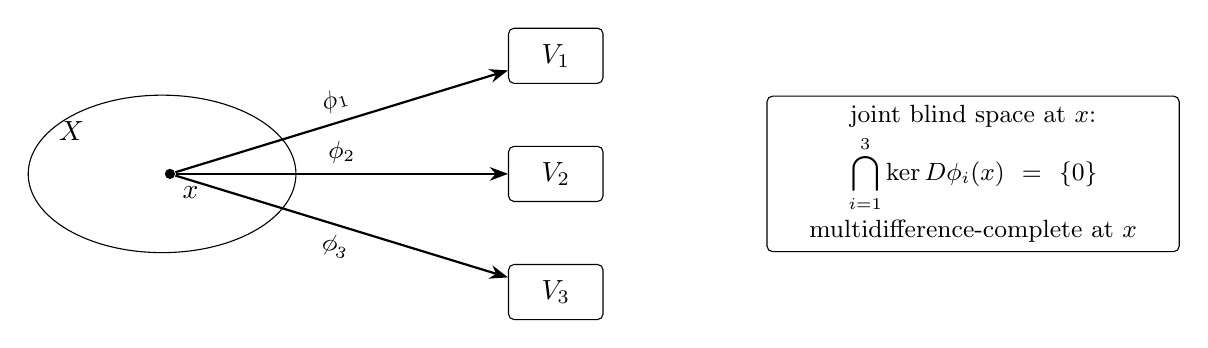
\begin{tikzpicture}[>=Stealth,
  box/.style={draw,rounded corners=2pt,minimum width=1.2cm,minimum height=0.7cm},
  pt/.style={circle,fill,inner sep=1.3pt}]
  \node[draw,ellipse,minimum width=3.4cm,minimum height=2.0cm] (X) at (0,0) {};
  \node at (-1.15,0.55) {$X$};
  \node[pt] (x) at (0.1,0) {}; \node[below right=1pt] at (x) {$x$};
  \node[box] (V1) at (5,1.5) {$V_1$};
  \node[box] (V2) at (5,0) {$V_2$};
  \node[box] (V3) at (5,-1.5) {$V_3$};
  \draw[->,thick] (x) -- node[above,sloped,font=\small] {$\phi_1$} (V1);
  \draw[->,thick] (x) -- node[above,font=\small] {$\phi_2$} (V2);
  \draw[->,thick] (x) -- node[below,sloped,font=\small] {$\phi_3$} (V3);
  \node[draw,rounded corners=2pt,text width=5.0cm,align=center,font=\small] at (10.3,0)
    {joint blind space at $x$:\\[2pt]
     $\displaystyle\bigcap_{i=1}^{3}\ker D\phi_i(x)=\{0\}$\\[2pt]
     multidifference-complete at $x$};
\end{tikzpicture}

\medskip
{\small (b)}
\caption{(a) The quadrilateral construction of this section, drawn with schematic curvilinear coordinate families. The chords $AB$ and $CD$ meet at $P$. The ratios $u=AP/AB$ and $v=DP/CD$ are the relational signature of $P$, and the affine map $\mathcal A^{-1}$ of Proposition~\ref{prop:recon} gives the interpolated coordinates. The interior coordinate curves are schematic and the positions of $A$, $B$, $C$, and $D$ are illustrative. (b) Several perspectives of one state. The family is multidifference-complete at $x$ when the intersection of their blind spaces is trivial (Section 3). Panel (b) restates the completeness condition of Section 3 for several perspectives of one state.}\label{fig:quad}
\end{figure}



\begin{definition}[Exact construction]
The construction is \emph{exact} if $\tilde\varphi=\varphi$ and $\tilde\lambda=\lambda$ on $\Omega$, that is, if $\varphi$ is affine in position along the selected vertical chords and $\lambda$ is affine along the selected horizontal chords. Its \emph{interpolation discrepancy} is $\delta(P)=|\varphi(P)-\tilde\varphi(P)|+|\lambda(P)-\tilde\lambda(P)|$.
\end{definition}

\begin{proposition}[Reconstruction]\label{prop:recon}
Let $\mathcal A:R\to[0,1]^2$ be the map
\[
\mathcal A(\lambda,\varphi)=\Bigl(\frac{\varphi-\varphi_-}{\varphi_+-\varphi_-},\ \frac{\lambda_+-\lambda}{\lambda_+-\lambda_-}\Bigr).
\]
Then $\mathcal A$ is an affine bijection with inverse $(u,v)\mapsto\bigl(\lambda_+-v(\lambda_+-\lambda_-),\ \varphi_-+u(\varphi_+-\varphi_-)\bigr)$, and $(\tilde\lambda,\tilde\varphi)=\mathcal A^{-1}\circ h$ on $\Omega$. Consequently $h(P)=h(Q)$ if and only if $(\tilde\lambda,\tilde\varphi)(P)=(\tilde\lambda,\tilde\varphi)(Q)$.
\end{proposition}

\begin{proof}
Each component of $\mathcal A$ is an affine function of one variable with nonzero slope, since $\varphi_-<\varphi_+$ and $\lambda_-<\lambda_+$, so $\mathcal A$ is a bijection onto $[0,1]^2$ with the stated inverse. The identity $(\tilde\lambda,\tilde\varphi)=\mathcal A^{-1}\circ h$ is the definition of the interpolated coordinates. Injectivity of $\mathcal A^{-1}$ gives the last statement.
\end{proof}

\begin{proposition}[Strong holography of the exact construction]\label{prop:holo}
If the construction is exact, then $h=\mathcal A\circ(\lambda,\varphi)$. Hence $h$ is injective on $\Omega$ if and only if $(\lambda,\varphi)$ is injective, and in that case $P=(\lambda,\varphi)^{-1}\bigl(\mathcal A^{-1}(h(P))\bigr)$. In the terminology of Section 4, $h$ is then strongly holographic with respect to equality.
\end{proposition}

\begin{proof}
Exactness says $(\tilde\lambda,\tilde\varphi)=(\lambda,\varphi)$, and Proposition~\ref{prop:recon} gives $(\tilde\lambda,\tilde\varphi)=\mathcal A^{-1}\circ h$, so $h=\mathcal A\circ(\lambda,\varphi)$. A composition with the bijection $\mathcal A$ is injective if and only if $(\lambda,\varphi)$ is. The reconstruction formula is the inverse of this factorization.
\end{proof}

A frame is therefore \emph{nondegenerate} in the relevant sense exactly when $\varphi_-\ne\varphi_+$, $\lambda_-\ne\lambda_+$, and $(\lambda,\varphi)$ is injective on $\Omega$. The last condition is what it means for the coordinates to be a chart on $\Omega$. The relational signature carries the same information as the chart, expressed relative to the frame in place of absolutely. Without exactness, injectivity of $h$ is by Proposition~\ref{prop:recon} the injectivity of the interpolated coordinates, a property of the chord rule that must be checked and is not guaranteed by the geometry of the frame.

The ratios are unchanged by the reparametrizations under which absolute values are arbitrary, and are changed by those under which they are not.

\begin{proposition}[Invariance and its limits]\label{prop:inv}
Let $u_\varphi(P)=(\varphi(P)-\varphi_-)/(\varphi_+-\varphi_-)$ denote the normalized coordinate ratio. (i) If $\varphi$ is replaced by $a\varphi+b$ with $a\neq0$, then $u_\varphi$ is unchanged, and likewise the analogue for $\lambda$. (ii) If $\psi=F(\varphi)$ with $F$ continuous and strictly monotone, then $u_\psi=G_F(u_\varphi)$, where
\[
G_F(u)=\frac{F\bigl(\varphi_-+u(\varphi_+-\varphi_-)\bigr)-F(\varphi_-)}{F(\varphi_+)-F(\varphi_-)}
\]
is a homeomorphism of $[0,1]$ fixing $0$ and $1$, and $G_F=\id$ if and only if $F$ is affine on $[\varphi_-,\varphi_+]$.
\end{proposition}

\begin{proof}
(i) The numerator and denominator of $u_\varphi$ are both multiplied by $a$ (with the endpoints' roles exchanged when $a<0$, which leaves the ratio unchanged). (ii) By definition $u_\psi=(F(\varphi)-F(\varphi_-))/(F(\varphi_+)-F(\varphi_-))$, and substituting $\varphi=\varphi_-+u_\varphi(\varphi_+-\varphi_-)$ gives $G_F(u_\varphi)$. Strict monotonicity of $F$ makes $G_F$ a strictly monotone continuous bijection of $[0,1]$ with $G_F(0)=0$ and $G_F(1)=1$. If $G_F=\id$ then $F$ is affine along the interval, and conversely.
\end{proof}

Proposition~\ref{prop:inv} identifies the transition map between two relational descriptions of one frame. Observers who differ by an affine change of coordinate agree on the ratios exactly, so nothing needs translating. Observers who differ by a nonlinear monotone change have relational coordinates related by $G_F$, and the disagreement is a homeomorphism of the unit interval fixing its endpoints. It is a translation with structure and not an error, in the sense of Section 5.

\section{Reading guide: what each result says and does not say}\label{sec:guide}

The table below lists the main results in order of appearance. The middle column restates each in words. The right column lists readings that go beyond it. Assumptions are those stated with the result, and none of the results is an empirical finding.

\begin{longtable}{@{}p{2.7cm}p{6.0cm}p{6.0cm}@{}}
\hline
\textbf{Result} & \textbf{Says} & \textbf{Does not say}\\
\hline
\endhead
Corollary~\ref{cor:dim} (dimension count) & A perspective whose feature space has fewer dimensions than the state space has a nonzero blind space at every point where it is differentiable. A locally constant perspective has a blind space equal to the whole tangent space. & That every measurement is blind, or that low dimension is the only source of blindness. A full-dimensional perspective can also have degenerate directions, as $x\mapsto x^3$ does at $0$.\\
Proposition~\ref{prop:open} (completeness is open) & If the joint differential is injective at a state, the joint observation map is injective near it, and completeness persists at nearby states. & Global injectivity. Nor is the converse asserted: local injectivity can hold where the differential fails to be injective.\\
Proposition~\ref{prop:frame} (frame characterization) & Completeness holds exactly when the frame operator is positive definite. The condition number is the ratio of the extreme sensitivities of the family. & That the condition number is intrinsic. It depends on the inner products chosen on the feature spaces, and it is not a measure of computational cost.\\
Proposition~\ref{prop:amp} (error amplification) & For a complete family, the least-squares estimate of a small displacement has error at most the noise size divided by the smallest singular value. & That the estimate fails in practice, or that noise is worst-case. The statement concerns the linearized estimate and is a bound.\\
Proposition~\ref{prop:hfacts} (holography facts) & A single holographic signature makes the family jointly holographic, and the converse fails. & That holography implies completeness or consistency, or the reverse.\\
Proposition~\ref{prop:tri} (trilateration) & In Euclidean space of dimension $m$, exact distances to $m+1$ affinely independent known points determine a point, and fewer landmarks do not in general. & How positioning systems work in practice, where distances are inferred from signals with unknown offsets. Nor does the count carry over to other geometries.\\
Proposition~\ref{prop:cocycle} and Proposition~\ref{prop:holbound} & Cocycle defects and holonomy discrepancies over a common state are bounded by accumulated pairwise discrepancies. & That vanishing holonomy implies vanishing discrepancy, since errors can cancel. The bounds concern loops over a common state.\\
Proposition~\ref{prop:trihol} (triangle holonomy) & For invertible transitions, holonomy around a triangle is trivial exactly when the cocycle defect vanishes. & Anything about loops that are not products of triangles.\\
Example~\ref{ex:winding} (winding) & Three charts on a circle can be exact on every overlap, satisfy every cocycle condition vacuously, and still have holonomy $2\pi$ around the loop. & That the holonomy is a computational error, or that no global chart exists. It obstructs a global \emph{linear} coordinate and disappears if a chart may take values in the circle.\\
Remark~\ref{rem:coh} (cohomology) & For group-valued transitions satisfying the cocycle condition, holonomy is classified by a cohomology class of the nerve of the cover. & A method for computing the class, or anything for transition maps that are not group-valued.\\
Proposition~\ref{prop:resid} (residual reduction) & At the population level, enlarging a chart by a new coordinate reduces the mean squared residual exactly when the residual is structured with respect to that coordinate. & That adding data helps in general. It says nothing about finite samples, where enlargement can fit noise.\\
Corollary~\ref{cor:growth} (limit of growth) & Under successive enlargement the mean squared residual is nonincreasing and converges to the residual of the limiting conditional expectation. & A stopping rule or a rate. The limit is zero only if the probe is measurable with respect to the limit.\\
Proposition~\ref{prop:indep} (independence) & The listed implications among (M), (H), (C), and (V) fail in general, each shown by an example. & That the properties are unrelated. Several relations hold, for instance completeness implies local injectivity of the joint map, and the triangle conditions control loops when the nerve is simply connected.\\
Proposition~\ref{prop:toolblind} (tool blind space) & Under assumptions A1 to A3, the blind directions of the fitted-parameter chart are those whose perceptual image is normal to the model manifold. & A claim about the geometry of any actual nervous system. The assumptions are stated and are strong.\\
Proposition~\ref{prop:branch}, Example~\ref{ex:mono}, Proposition~\ref{prop:wellfn} & With a non-injective immersion, the fit is multivalued and the blind space depends on the branch. A fitted function descends to the chart only if it is constant on the fibers of the renderer. & That any fitted parameter of any instrument is meaningless. They give tests for when a parameter is a well-defined coordinate.\\
Contaminated growth (Section 8) & If exposure changes how experiences are reported, residuals under different reference laws are not comparable. & That exposure does change reports. That is left as an empirical question.\\
Propositions~\ref{prop:recon} to \ref{prop:inv} (quadrilateral) & The ratios along chords determine the interpolated coordinates by an affine bijection, and the signature is injective exactly when the coordinates form a chart. & That the interpolated coordinates equal the true coordinates without exactness, or anything about interpolation rules other than affine along chords.\\
\hline
\end{longtable}

\section{Worked examples with numbers}\label{sec:examples}

This section works small cases in full. The purpose is to fix what the definitions mean before they are used, and to show in each case where a tempting extrapolation would fail.

\subsection{Three instruments on a position in space}

Let $X=\R^3$ with points $x=(x_1,x_2,x_3)$. Take two instruments,
\[
\phi_A(x)=(x_1,x_2),\qquad \phi_B(x)=(x_2,x_3).
\]
The differential of $\phi_A$ is the matrix with rows $e_1,e_2$, so its blind space is $\N_A=\mathrm{span}\{e_3\}$, of dimension $1=3-2$ as Corollary~\ref{cor:dim} requires. The differential of $\phi_B$ has rows $e_2,e_3$, so $\N_B=\mathrm{span}\{e_1\}$. Each instrument alone is blind, and $\N_A\cap\N_B=\{0\}$, so the pair is complete. The stacked Jacobian has rows $e_1,e_2,e_2,e_3$, and the frame operator is $S=\mathrm{diag}(1,2,1)$, so $\kappa_{\mathrm{obs}}=\sqrt{2/1}\approx1.41$. The pair is well conditioned.

Now replace $B$ by an instrument that looks along nearly the same axis as $A$:
\[
\phi_{B,\epsilon}(x)=(x_1,\ x_2+\epsilon x_3),\qquad \epsilon>0 .
\]
The rows of the stacked Jacobian are $e_1,e_2,e_1,e_2+\epsilon e_3$, and
\[
S=\begin{pmatrix}2&0&0\\0&2&\epsilon\\0&\epsilon&\epsilon^2\end{pmatrix},
\qquad
\lambda_\pm=\frac{2+\epsilon^2\pm\sqrt{4+\epsilon^4}}{2}
\]
are the eigenvalues of its lower block, the remaining eigenvalue being $2$. For $\epsilon>0$ the family is complete, since $\det S=2\epsilon^2>0$. At $\epsilon=0$ the rows repeat and the blind space $\mathrm{span}\{e_3\}$ returns. For small $\epsilon$, $\sigma_{\min}^2=\lambda_-\approx\epsilon^2/2$ and $\sigma_{\max}^2=\lambda_+\approx2$, so $\kappa_{\mathrm{obs}}\approx2/\epsilon$. For $\epsilon=0.01$ this is about $200$, and by Proposition~\ref{prop:amp} noise of size $\|\eta\|$ can be amplified to an error of about $\sqrt2/\epsilon\approx141$ times $\|\eta\|$ in the direction $e_3$.

Two cautions. First, the numbers depend on the weights. Rescaling the outputs of one instrument changes $S$ and hence $\kappa_{\mathrm{obs}}$, though it does not change whether the family is complete. Second, the museum picture, in which one camera covers the door and another the hallway, is a picture of \emph{places}. A blind space is a set of \emph{directions of change} in the state, not a region that an instrument cannot see. The picture is useful for the idea that blind spaces of different instruments can cancel, and it should not be pressed further.

\subsection{A discrete category}

Let $X=\R$ and let a perspective report a label: $\phi(x)=1$ if $x\ge c$ and $\phi(x)=0$ otherwise, for a cutoff $c$. At every $x\neq c$ the map is locally constant, so $D\phi(x)=0$ and $\N(x)=\R$. The label is blind, to first order, to every change of $x$ that does not cross the cutoff. At $x=c$ the map is not differentiable, so the differential-based machinery of Section 3 says nothing there, and the metric machinery of Section 5 is the appropriate one.

The statement is about the label. If another perspective records $x$ itself, that perspective is not blind to these changes, and the pair can be complete. Nor does the example say that discretization is always harmful or that any particular field of measurement relies on labels. It says only that a family made entirely of locally constant perspectives cannot be multidifference-complete (Corollary~\ref{cor:dim}).

\subsection{Landmarks on a line and on a circle}

On $X=\R$ with one landmark $\ell$, the signature $\sigma(x)=|x-\ell|$ takes the same value at $\ell+d$ and $\ell-d$, so it is not injective. With two distinct landmarks it is, in agreement with Proposition~\ref{prop:tri} for $m=1$. In $\R^3$ four affinely independent landmarks are needed and three leave a reflection.

On the circle $S^1=\R/2\pi\mathbb Z$ with arc-length distance, take the landmarks $0$ and $\pi$. For $x\in(-\pi,\pi]$ the signature is $(|x|,\ \pi-|x|)$, so $x$ and $-x$ have the same signature and the signature is not injective. Two landmarks that are neither equal nor antipodal do separate all points (Section 4). The counts in this essay assume exact distances to known points. Practical positioning systems infer distances from signals with an unknown receiver offset, which requires one more measurement, and that is a different problem from the one treated here.

\subsection{Three charts on a circle, with numbers}

Take $\epsilon=\pi/6$ in Example~\ref{ex:winding}. The three arcs are $U_1=(-\pi/6,5\pi/6)$, $U_2=(\pi/2,3\pi/2)$, and $U_3=(7\pi/6,13\pi/6)$, each read as an interval of angles. The overlaps are $U_{12}=(\pi/2,5\pi/6)$, $U_{23}=(7\pi/6,3\pi/2)$, and $U_{13}$, which is the arc around angle $0$, read as $(-\pi/6,\pi/6)$ in chart $1$ and as $(11\pi/6,13\pi/6)$ in chart $3$. The transition maps, extended to all of $\R$, are $T_{21}=T_{32}=\mathrm{id}$ and $T_{31}(y)=y+2\pi$. On each overlap they agree exactly with the charts, so every local discrepancy is zero.

Follow a reading around the loop $1\to2\to3\to1$. Start with $y=0$ in chart $1$. Chart $2$ reads $0$, chart $3$ reads $0$, and returning to chart $1$ applies $T_{13}(y)=y-2\pi$, giving $-2\pi$. The reading has changed by $2\pi$ though every step was exact. Nothing was miscalculated. The atlas records a fact about the circle that no single chart contains. If one chart were allowed to take values in the circle $\R/2\pi\mathbb Z$, that chart would cover the whole space and the shift would disappear. What the winding obstructs is an atlas of \emph{linear} coordinates.

\subsection{A structured and an unstructured residual}

Let $X=[0,1]^3$ with the uniform distribution, chart $\phi(x)=x_1$, and probe $P(x)=x_1+x_2$. Then $\E[P\mid\phi]=x_1+\tfrac12$, so the residual is $\varepsilon=x_2-\tfrac12$ with mean squared value $\mathrm{Var}(x_2)=1/12$.

Enlarge the chart by $z=x_2$. Then $\E[P\mid\phi,z]=P$ and the residual is zero. The reduction is $1/12$, equal to $\E\bigl[(\E[P\mid\phi,z]-\E[P\mid\phi])^2\bigr]=\E[(x_2-\tfrac12)^2]$, as Proposition~\ref{prop:resid} states. The residual was structured with respect to $z$.

Enlarge instead by $w=x_3$, which is independent of $P$. Then $\E[P\mid\phi,w]=\E[P\mid\phi]$, the two conditional expectations coincide, and the mean squared residual stays at $1/12$. The residual is unstructured with respect to $w$. The example is population-level. In a finite sample, adding $w$ could reduce the observed residual by fitting noise, which the proposition does not address.

\section{Terms, ambiguities, and conventions}\label{sec:terms}

\subsection{Glossary}

The entries restate definitions given earlier and say where each is used. A definition in the text governs if the two differ.

\begin{description}[leftmargin=1.2em,style=nextline,itemsep=3pt]
\item[State space $X$.] The set of states being measured. Where derivatives are used it is a smooth manifold of dimension $m$; where probabilities are used it carries a probability measure. It is a modeling object, and no claim is made that any particular phenomenon is a manifold.
\item[Perspective, chart, observation map.] A triple $(U_\alpha,V_\alpha,\phi_\alpha)$: a domain in $X$, a feature space, and a map from the domain to the feature space. ``Chart'' is used for a perspective when the emphasis is on coordinates. ``Observer'' is used only informally and carries no claim about awareness.
\item[Feature space.] The set of values a perspective can report, whether or not every value corresponds to a state.
\item[Blind space.] The kernel of the differential of an observation map at a state: the directions of change to which the perspective is insensitive to first order. The \emph{joint} blind space is the intersection of the blind spaces of all perspectives containing the state.
\item[Multidifference completeness.] The joint blind space is $\{0\}$ at a state. Equivalently, the joint observation map is an immersion there. It concerns \emph{infinitesimal directions of change}, not distinctions between far-apart states.
\item[Frame operator and condition number.] The sum of the operators $D\phi_\alpha^{*}D\phi_\alpha$ and the ratio of the extreme singular values of the stacked differential. Both depend on the inner products chosen.
\item[Signature.] A map from states to a space of relational descriptions, for instance distances to landmarks or ratios along chords. It is \emph{strongly holographic} for an equivalence relation $\sim$ if equal signatures imply equivalent states, and \emph{jointly holographic} if the family of signatures does.
\item[Transition map.] A map $T_{\beta\alpha}$ from the feature space of one perspective to that of another, intended to satisfy $\phi_\beta=T_{\beta\alpha}\circ\phi_\alpha$ on overlaps.
\item[Transition discrepancy.] The distance $\delta_{\alpha\beta}(x)$ between the reading of $\beta$ at $x$ and the translation of the reading of $\alpha$. A discrepancy is a measurement of disagreement and is not by itself an error.
\item[Cocycle defect.] For a triple of perspectives, the distance between translating through the middle one and translating directly.
\item[Holonomy map and discrepancy.] The composite of the transition maps around a loop of perspectives, and its distance from the identity at a given state. Three situations are distinguished in the text: holonomy over a common state, bounded by discrepancies (Proposition~\ref{prop:holbound}); topological holonomy such as the winding of Example~\ref{ex:winding}; and gauge holonomy from redundant parameters (Example~\ref{ex:mono} and the gauge example of Section 8).
\item[Atlas, enriched atlas, holocoordinate system.] An atlas is a family of charts with transition maps. An enriched atlas adds relational signatures and residuals, and a holocoordinate system is an enriched atlas (Definition~\ref{def:holo}). The word ``atlas'' is used in its technical sense throughout.
\item[Probe, residual.] A probe is a real-valued property of a state. The residual of a chart for a probe is the difference between the probe and its best prediction from the chart, in the sense of conditional expectation.
\item[Structured residual.] A residual whose conditional expectation given the enlarged chart differs from that given the original chart (Proposition~\ref{prop:resid}).
\item[Exact construction.] In Section~\ref{sec:quad}, one for which the interpolated coordinates equal the true coordinates.
\end{description}

\subsection{Ambiguities and how they are resolved}

\begin{enumerate}[label=(\alph*),nosep]
\item \emph{``Difference''.} The word can mean a distinction between two states or an infinitesimal direction of change. The essay uses the second in Section 3, so ``multidifference'' refers to combining the directions of change registered by several perspectives.
\item \emph{``Complete''.} Three things could be meant: that the joint blind space is trivial (multidifference completeness), that a signature determines the state (holography), or that the charts cover the state space. The essay uses ``complete'' only for the first, and uses ``holographic'' for the second.
\item \emph{``Consistent''.} Transition consistency (C) means that all discrepancies vanish on overlaps and all cocycle conditions hold. It is stronger than agreement on the data actually collected.
\item \emph{``Holonomy''.} A global shift accumulated around a loop can come from topology, from redundant parameters, or from accumulated pairwise discrepancy. The essay names these separately and treats only the first two as properties of the atlas independent of measurement error.
\item \emph{``Local'' and ``global''.} Completeness is local and first-order. Injectivity of a signature can be local or global. The cocycle condition is a condition on triples, while holonomy concerns loops, and a loop need not be a product of triangles.
\item \emph{``Space''.} The state space is not assumed to be Euclidean. ``Non-Euclidean'' here describes a geometry in the technical sense, for instance the circle, and the essay makes no claim about whether any space of beliefs or experiences is non-Euclidean.
\item \emph{``Error''.} A discrepancy, residual, or holonomy is a datum of the atlas. Whether it reflects an error of measurement, a missing coordinate, or a feature of the space is the question the atlas is built to pose.
\item \emph{``Proved''.} Every proposition is proved under the assumptions stated with it. Where an application uses a proposition, the application inherits those assumptions.
\item \emph{``Independent''.} In Proposition~\ref{prop:indep}, independence of properties means that particular implications fail in some model. It does not mean that no relations hold.
\end{enumerate}

\subsection{Conventions and notation collisions}

Norms and inner products on tangent and feature spaces are chosen and reported; completeness does not depend on them, while conditioning does. Sections 8 and 9 reuse symbols: in Section 8, $\phi_\tau$ is the tool chart and $\theta$ a parameter vector, and in Section 9, $\varphi$ and $\lambda$ are the two coordinate functions of a quadrilateral frame and are not observation maps $\phi_\alpha$. The symbol $R$ denotes a renderer in Section 8 and the coordinate rectangle in Section 9. The symbol $\pi$ denotes the nearest-point retraction in Section 8. Where a symbol is reused, the local definition governs.

\section{Common misreadings}\label{sec:mis}

The following statements are frequently drawn from summaries of the essay. Each is followed by the correction and a pointer to the relevant result.

\begin{enumerate}[label=\textbf{M\arabic*.},leftmargin=2.2em,itemsep=4pt]
\item \emph{``Every simple coordinate is guaranteed to have a blind spot.''} Blindness is guaranteed only in two situations: the feature space has fewer dimensions than the state space, or the perspective is locally constant (Corollary~\ref{cor:dim}). A perspective of full dimension can be complete on its own. The essay gives no argument that measurements in general are blind.
\item \emph{``A blind space means the instrument is bad.''} A blind space is a set of directions and is a property of an observation map and a state space. A well-made instrument can have a large blind space because it reports few quantities.
\item \emph{``Two cameras that together cover a room remove the blind space.''} Blind spaces are directions of change, not regions of space. Two instruments can cancel each other's blind directions, but the picture of cameras covering places is only an analogy (Section~\ref{sec:examples}).
\item \emph{``A complete family is a good family.''} Completeness says only that the joint kernel is trivial. A complete family can be nearly incomplete, and then errors are amplified (Proposition~\ref{prop:amp}, Section~\ref{sec:examples}).
\item \emph{``The condition number measures how hard the system has to compute.''} It measures the ratio of the largest to the smallest sensitivity of the family to changes of state. It is not a measure of computational cost, and it depends on the weights chosen.
\item \emph{``Holographic means complete, or consistent, or correct.''} It means that a signature determines the state up to the chosen equivalence, and nothing more (Proposition~\ref{prop:hfacts}). It is used here in a reconstructive sense unrelated to the holographic coordinate of high-energy physics (Remark~\ref{rem:term}).
\item \emph{``Three or four landmarks always suffice.''} $m+1$ affinely independent landmarks with exact distances suffice in Euclidean $\R^m$ (Proposition~\ref{prop:tri}). In other geometries injectivity must be checked, and two antipodal landmarks fail on a circle. The count is not a description of how real positioning works.
\item \emph{``Discrete categories are always harmful.''} A family made entirely of locally constant perspectives cannot be complete. The statement concerns the label and first-order sensitivity, and a family that also records the underlying quantity is not affected.
\item \emph{``If local translations agree, the whole system is consistent.''} For triangles, the triangle holonomy vanishes exactly when the cocycle defect does (Proposition~\ref{prop:trihol}), and when the nerve of the cover is simply connected the triangle conditions control every loop (Remark~\ref{rem:coh}). The winding example shows that loops around a hole in the nerve are not controlled by local agreement.
\item \emph{``Holonomy means someone made a mistake.''} Topological holonomy and gauge holonomy are not mistakes. Holonomy \emph{discrepancy} accumulated over a common state is bounded by pairwise discrepancies, and those may reflect error, missing coordinates, or genuine differences between perspectives (Proposition~\ref{prop:holbound}).
\item \emph{``The winding means a global chart is impossible.''} It means a global chart with values in a \emph{linear} space is impossible for that cover. A chart valued in the circle exists.
\item \emph{``Adding more variables improves a model.''} At the population level a residual is reduced exactly when it is structured with respect to the added coordinate (Proposition~\ref{prop:resid}). Adding an unstructured variable does nothing at that level. In finite samples it can appear to help by fitting noise.
\item \emph{``The growth rule tells you when to stop.''} It does not. The mean squared residual is nonincreasing and converges (Corollary~\ref{cor:growth}), but no rate or stopping criterion is given, and the limit is zero only if the probe is measurable with respect to the limiting information.
\item \emph{``The four properties are unrelated.''} Proposition~\ref{prop:indep} lists particular non-implications. Relations do hold: completeness implies local injectivity of the joint map, triangle conditions control loops when the nerve is simply connected, and exactness implies vanishing holonomy discrepancy over a common state.
\item \emph{``The tracer tool maps the geometry of the visual cortex.''} Section 8 treats an instrument as a chart under stated modeling assumptions and derives its blind space within them. The fitted parameters are coordinates of the instrument. Nothing in the essay identifies them with neural quantities, and criteria for doing so are stated as conditions (Section 8).
\item \emph{``The essay shows that exposure to the tool changes people's memories.''} It states only that if reports change with exposure, residuals under different reference laws are not comparable. Whether they do is an empirical question left open.
\item \emph{``Residual zero means the model is true.''} It means the probe is predicted exactly by the chart at the population level. The chart may still be blind to other properties.
\item \emph{``The essay applies to finance, medicine, organizations, or consciousness.''} No such application is made. Where the text or an informal summary uses examples from those areas, they are illustrations of the mathematics and carry no evidential weight.
\end{enumerate}

\section{Scope and limits}\label{sec:scope}

The results above are conditional on structure that must be argued for in any application.

First, the differential-geometric statements require that $X$ be a smooth manifold and the $\phi_\alpha$ differentiable. For state spaces of experience or of relational configuration this is a modeling hypothesis, not a finding. Where it fails, the algebraic content of Sections 5 through 7 survives, since it uses only metrics and Lipschitz maps, while Section 3 must be replaced by a discrete or set-theoretic analogue of distinguishability.

Second, the derivatives $D\phi_\alpha(x)$ are not observable from finitely many reports. In practice they would be approximated by finite differences over nearby states, and the completeness criterion becomes a statement about the numerical rank of an estimated Jacobian, with the stability caveats of Section 3.

Sections 10 to 13 add no results. They restate, illustrate, and delimit the results of the earlier sections, and where a summary in them is shorter than the corresponding proposition, the proposition governs.

Section 9 assumes a rule selecting a chord through each point and, for exactness, an affine interpolation hypothesis along the chords. Without them the ratios need not be functions of the point, and the relation between the ratios and the coordinates is only that of the interpolated coordinates to the true ones.

Third, completeness at first order is a local and infinitesimal property. It does not guarantee global injectivity of the joint observation map, and it says nothing about whether the perspectives span the phenomenon rather than the instrument. A coordinate fitted within a family of charts is first of all a coordinate of that family; the growth rule of Section 6 is the mechanism by which persistent, structured failure can extend the family, and the limit in Corollary~\ref{cor:growth} states exactly which residual survives when the added coordinates are exhausted.

\newpage
\begin{thebibliography}{9}
\bibitem{lee} Lee, J. M. (2013). \emph{Introduction to Smooth Manifolds} (2nd ed.). Springer.
\bibitem{christensen} Christensen, O. (2003). \emph{An Introduction to Frames and Riesz Bases}. Birkh\"auser.
\bibitem{golub} Golub, G. H., and Van Loan, C. F. (2013). \emph{Matrix Computations} (4th ed.). Johns Hopkins University Press.
\bibitem{bott} Bott, R., and Tu, L. W. (1982). \emph{Differential Forms in Algebraic Topology}. Springer.
\bibitem{williams} Williams, D. (1991). \emph{Probability with Martingales}. Cambridge University Press.
\bibitem{qri_note} Qualia Research Institute. \emph{Tracer Replication Tool} (Psychophysics Toolkit), and accompanying writeup by A.\ G\'omez Emilsson and colleagues. \url{https://qri.org}.
\bibitem{maldacena} Maldacena, J. (1998). The large $N$ limit of superconformal field theories and supergravity. \emph{Advances in Theoretical and Mathematical Physics}, 2, 231--252.
\bibitem{susskind} Susskind, L., and Witten, E. (1998). The holographic bound in anti-de Sitter space. arXiv:hep-th/9805114.
\bibitem{coons} Coons, S. A. (1967). \emph{Surfaces for Computer-Aided Design of Space Forms}. MIT Project MAC Technical Report MAC-TR-41.
\bibitem{flyxion} Flyxion. \emph{Rehearsable Abstraction: Editable Expansion as a Regime of Implementation Visibility}. Unpublished essay, 2026.
\end{thebibliography}

\end{document}

